%%%%%%%%%%%%%%%%%%%% chapter2.tex %%%%%%%%%%%%%%%%%%%%%%%%%%%%%%%%%
%
\chapter{Kinematics in One and Two Dimensions}
\label{ch-kinematics} % Always give a unique label
In almost all introductory physics courses, we begin with kinematics in one and two dimensions. We will begin our study of computational physics similarly, as we can easily check our code in the limiting case of no air resistance and constant vertical acceleration. We will also explore realms that are generally not discussed: motion with linear and non-linear air resistance, and motion with non-constant vertical acceleration. 
\section{Motion in one dimension: Linear Air Resistance}
\label{sec-1d}
Consider the simplest case of a ball dropped from rest from close to the surface of Earth. Assuming that the ball is sufficiently dense, so that we can ignore buoyancy, the main forces on the ball during its downward flight are gravitation and air resistance. If we choose positive y upward, and y=0 at the ground, then Newton's second law tells us that 
$$ - F_g + F_d = - m a_y ,$$
where $F_g$ and $F_d$ are the magnitudes of the gravitational force and the drag force, respectively, and $a_y$ is the \textit{magnitude} of the acceleration of the ball. The free-body diagram is shown in  Figure~\ref{fig-FreeFall}. 
\begin{figure}
\centering
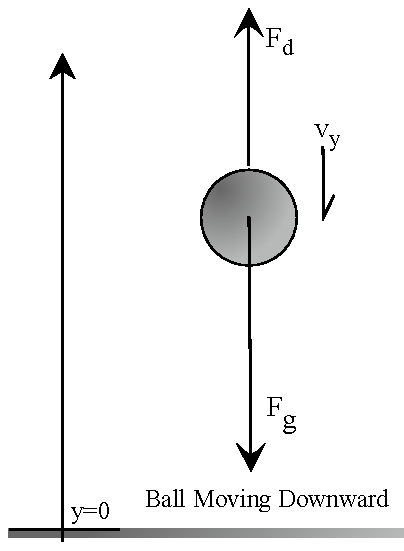
\includegraphics[height=6cm]{Figures/5Kinematics/FreeFallDown}
\caption{Free body diagram for an object released from rest a short distance above the surface of Earth.}
\label{fig-FreeFall}       % Give a unique label
\end{figure}
\subsection{Theoretical Picture}
\label{sec-LinDragTheory}
The drag force $F_d$ is actually a complicated force that depends on the shape of the object, its speed, and the density of the air and only in simple situations can we \textbf{analytically} calculate its exact form. We begin by working out one such case; we assume that the drag force is proportional to the speed of the ball (this is only good for very small velocities; realistic projectiles dropped from appreciable heights are better modeled by air resistance that is proportional to the square of the speed). Then we can write the equation of motion for the ball as 

$$- m g + b v_y = m(a_y),$$
where $a_y$ is the acceleration of the ball as it falls. Now, multiplying by $-1/m$,
$$ g - \frac{b}{m} v_y = -a_y .$$
Since the acceleration is the derivative of the velocity, and the velocity is increasing in the negative directions, $a_y = -\frac{dv}{dt}$, and we can write this as 
\begin{equation}
	g - \frac{b}{m} v_y = \frac{d v_y}{dt}
	\label{eq-diffeqLinDrag}
\end{equation}
Then, multiplying by $dt$ and dividing by $g - \frac{b}{m} v_y$, we have
$$
	\frac{dv_y}{g - \frac{b}{m} v_y} = dt
$$
This equation can be easily integrated to yield 
$$
-\frac{m}{b}\ln\left(g - \frac{b}{m} v_y\right) = t + const
$$
or, using the properties of the logarithm, the speed of the ball is 
\begin{equation}
v_{y} (t) = \frac{mg}{b}\left(1-\frac{A}{g}e^{-\frac{b}{m}t}\right)
\label{eq:VvsT_LinDrag1}
\end{equation}
where $A$ is some constant. We determine the constant $A$ by the initial condition $v_y(0) = 0$, and this implies that $A=g$; hence Equation~\ref{eq:VvsT_LinDrag1} simplifies to
\begin{equation}
v_{y} (t) = \frac{mg}{b}\left(1-e^{-\frac{b}{m}t}\right)
\label{eq:VvsT_LinDrag2}
\end{equation}
If the object falling falls for a sufficiently long time, then the air resistance will continue to increase as its speed increases, and at some point, the air resistance will be equal in size to the gravitational pull on the object; at this point, the net force will be zero, and the object will fall at a constant rate referred to as its terminal velocity, $v_t$. 

Looking at Equation~\ref{eq:VvsT_LinDrag2} in the limit $t\rightarrow \infty$, we find that 
\begin{equation}
v_t = \frac{mg}{b}
\label{eq:terminal_v}
\end{equation}
and hence, the speed of the falling object as a function of time may also be written as 
\begin{equation}
v_{y} (t) = v_{t} \left(1-e^{-\frac{gt}{v_{t}}}\right)
\label{eq:VvsT_LinDrag3}
\end{equation}
\begin{figure}[t]
\centering
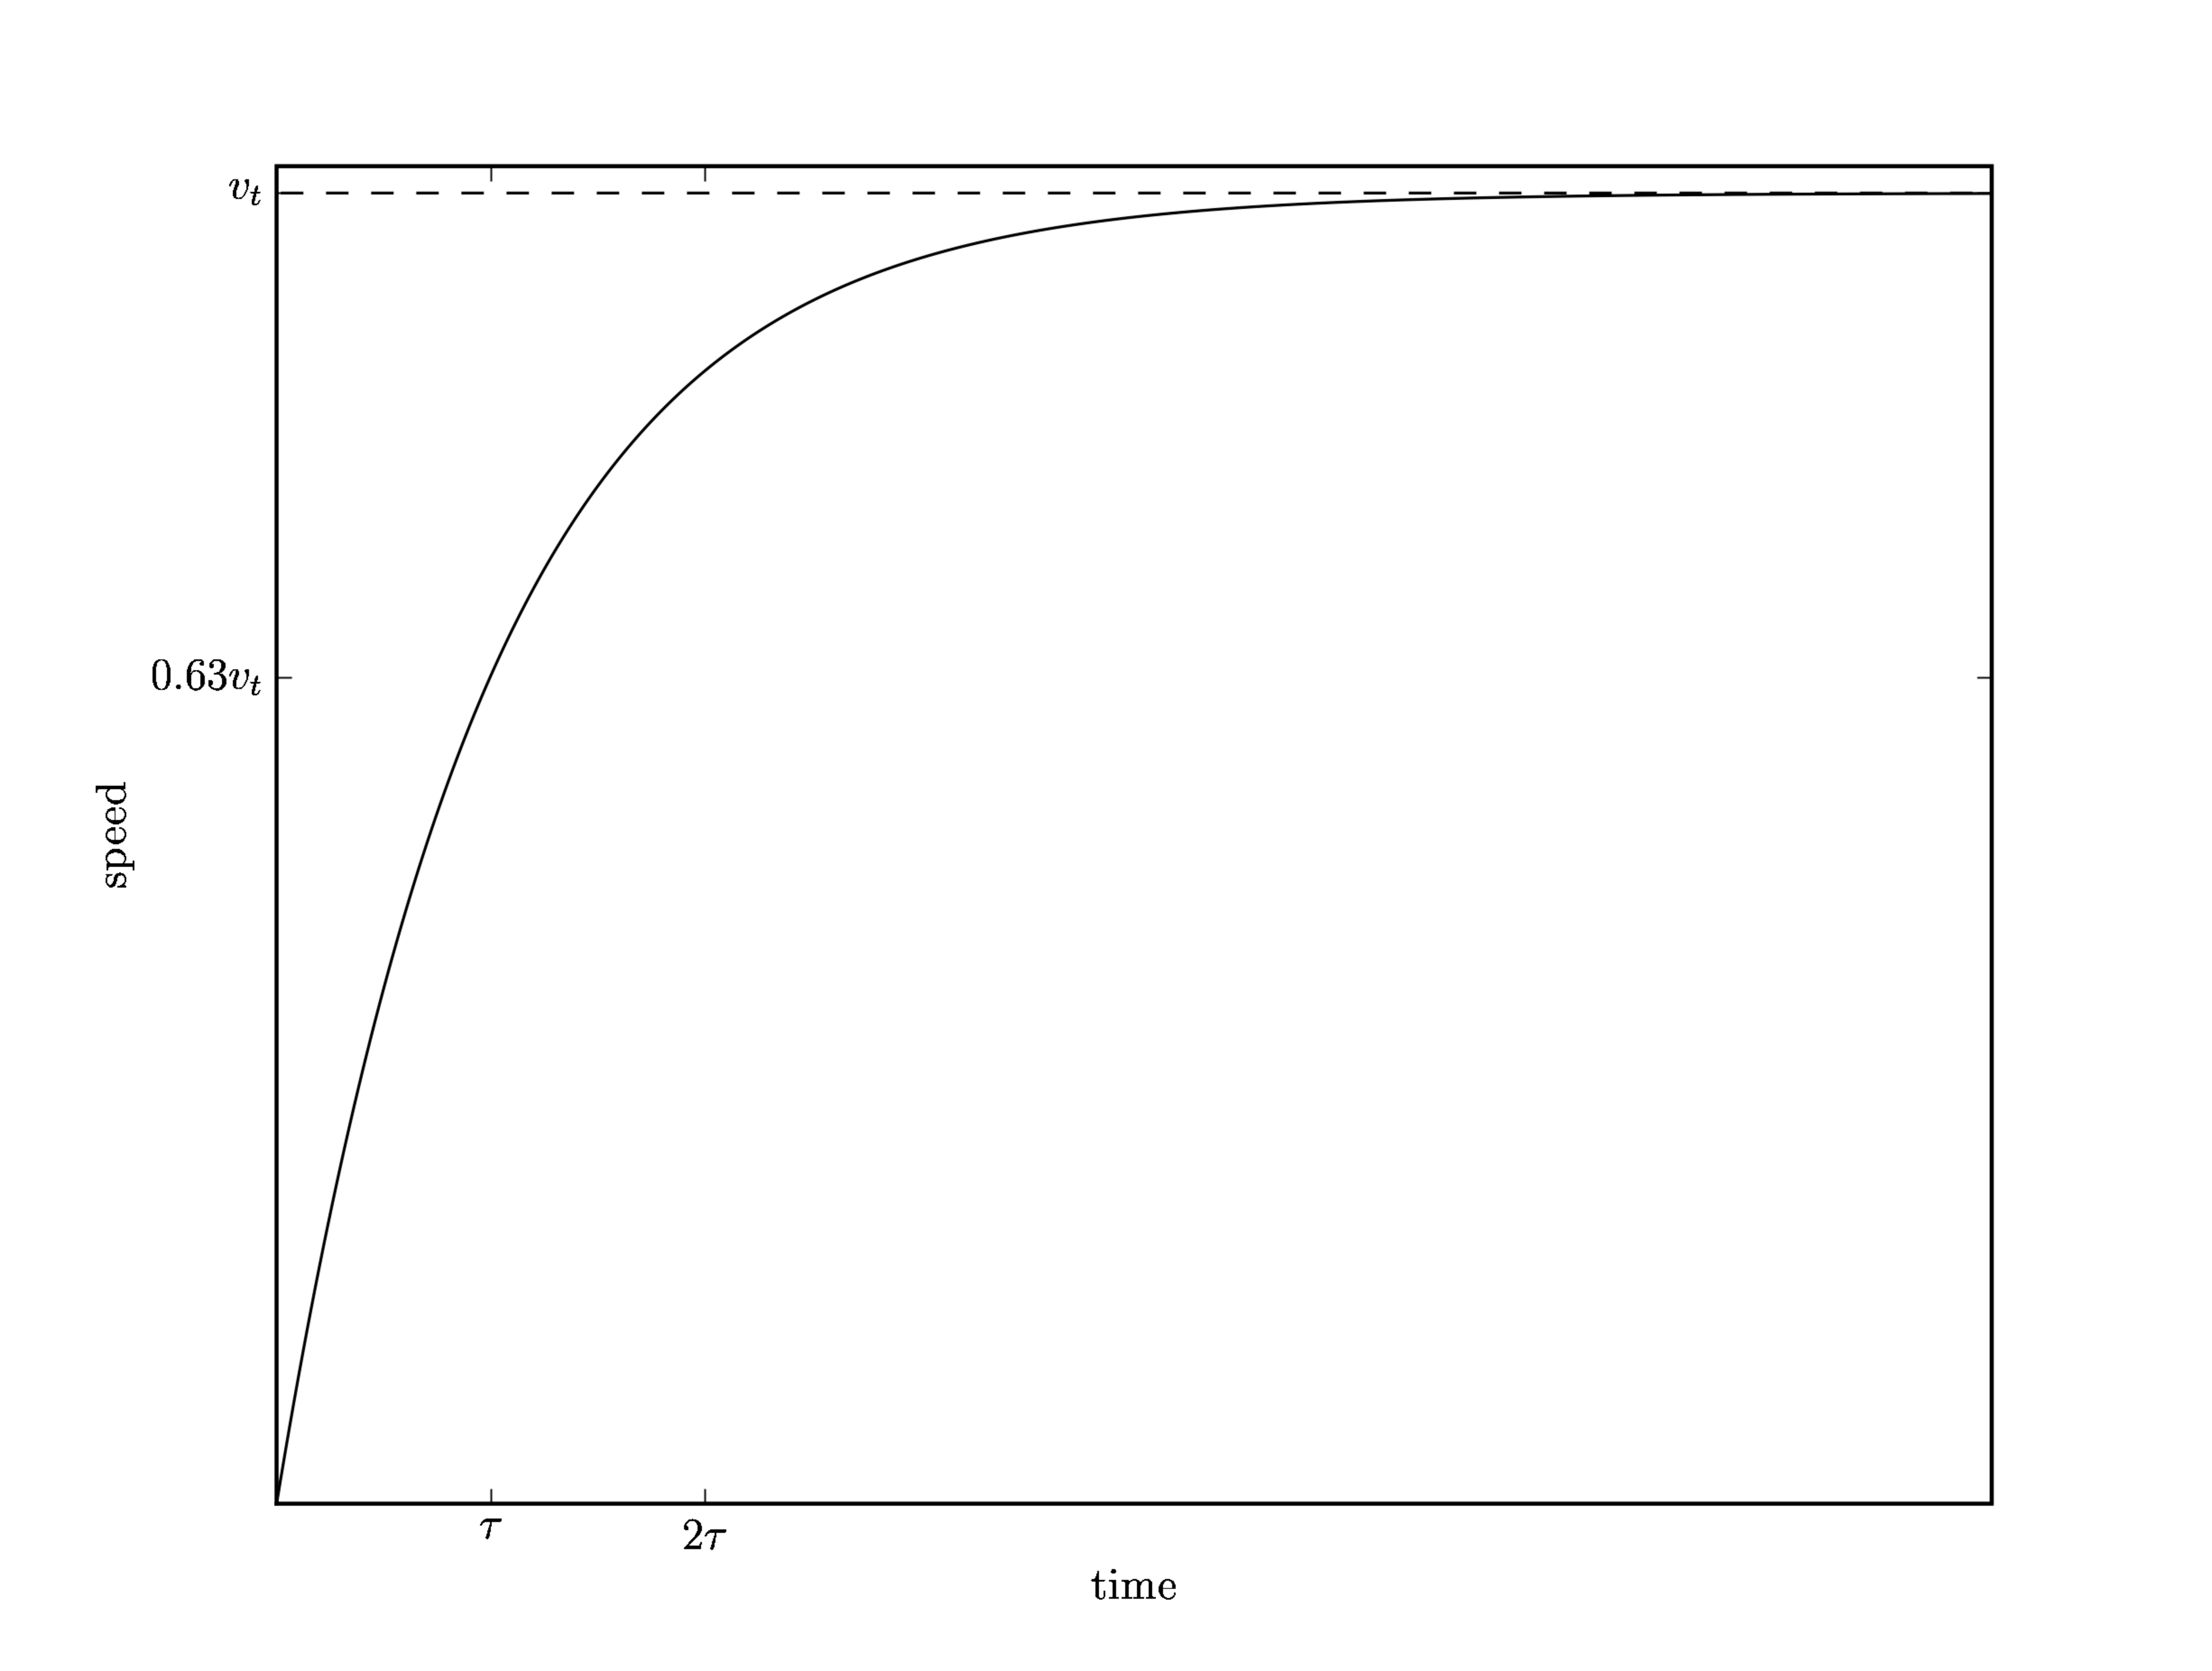
\includegraphics[height=7cm]{Figures/5Kinematics/LinearDragSpeed}
\caption{Speed vs time for an object falling in a linear drag regime. Notice that if we define a time constant $\tau = v_t/g$, the object reaches 63\% of its terminal velocity after $\tau$ seconds. After several time constants have elapsed, the object is very close to its terminal velocity.}
\label{fig-LinearDrag}       % Give a unique label
\end{figure}
Notice that if we define a time constant $\tau = v_{t}/g$, we can write this as
\begin{equation}
v_{y} (t) = v_{t} \left(1-e^{-\frac{t}{\tau}}\right)
\label{eq:VvsT_LinDrag4}
\end{equation}
and then, when $t=\tau$, the speed will be $v_{y} (t=\tau) = v_{t} \left(1-e^{-1}\right)\approx 0.63v_t$. After two time constants, the speed will be at $\approx 0.86v_t$. After four time constants, the speed will be within 2\% of its terminal value. This can be seen in Figure~\ref{fig-LinearDrag}

\subsection{Simulation of Linear Drag}
\label{sec-LinDragSimulation}
Now, suppose we want to simulate the free fall motion of the ball that we've just analytically discussed. To do so, we begin with Newton's equation of motion for the ball (Equation~\ref{eq-diffeqLinDrag}) 
\begin{equation}
	\frac{d v_y}{dt} = g - \frac{b}{m} v_y,
	\label{eq-diffeqEuler}
\end{equation}
and multiply both sides by dt:
$$ d v_y = \left(g - \frac{b}{m} v_y\right) dt.$$
then, we \textbf{approximate} the change in $v_y$ by 
$$\Delta v_y \approx \left(g - \frac{b}{m} v_y\right) \Delta t.$$
A more convenient form to write this in is to use the definition of the terminal velocity (Equation~\ref{eq:terminal_v}) to write this as
\begin{equation}
	 \Delta v_y \approx g\left(1 - \frac{v_y}{v_t}\right) \Delta t.
\end{equation}
This is the form we will use to numerically integrate the equation of motion.
If we are given the initial velocity in the vertical direction as $v_{y}(0)$, then a time $\Delta t$ later, the velocity is 
$$v_y(\Delta t) \approx v_{y}(0)+ \Delta v_y,$$
or 
$$v_y(\Delta t) \approx v_{y}(0) + g\left(1 - \frac{v_{y}(0)}{v_t}\right) \Delta t $$
notice that we are using the value of the known initial velocity to determine the velocity at the next time step. In a similar fashion, the velocity after one more time step is 
$$v_y(2\Delta t) \approx v_{y}(\Delta t) + g\left(1 - \frac{v_{y}(\Delta t)}{v_t}\right) \Delta t. $$
The value of the velocity at the next time step is the value at the previous step, plus the dervivative $\frac{dv}{dt}$ evaluated at this previous time step times $\Delta t$. This is called the \textbf{Euler Method}, and is the simplest method for numerically solving a differential equation. Soon, we will see its origins and its limitations; for now, here is a piece of Python code to solve for the speed of the dropped ball using linear air drag:
\pagebreak

\lstinputlisting[caption={This program uses the Euler method to solve for the velocity of a ball falling under the influence of a drag force proportional to the speed of fall. It also plots the analytic solution for comparison purposes.}, label=code:FreeFallLinearDrag, frame=single]{Code/5Kinematics/FreeFall_V.py}
Here is the file EulerFreeFall.py, which contains the functions that implement the Euler method:
\lstinputlisting[caption={The contents of the file EulerFreeFall.}, label=code:EulerFreeFall, frame=single]{Code/5Kinematics/EulerFreeFall.py}

For a ball bearing of diameter 1.25 cm falling in glycerin, the terminal velocity is roughly 0.2 m/s (see ~\cite{Baamann:2002}). If we run the script in Listing~\ref{code:FreeFallLinearDrag} with 
\begin{itemize}
	\item vinitial = 0.0
	\item vterminal = 0.2
	\item  tmax=0.2
	\item dt=0.01
\end{itemize}
we obtain the output shown in Figure~\ref{fig:glycerin}.
\begin{figure}
\centering
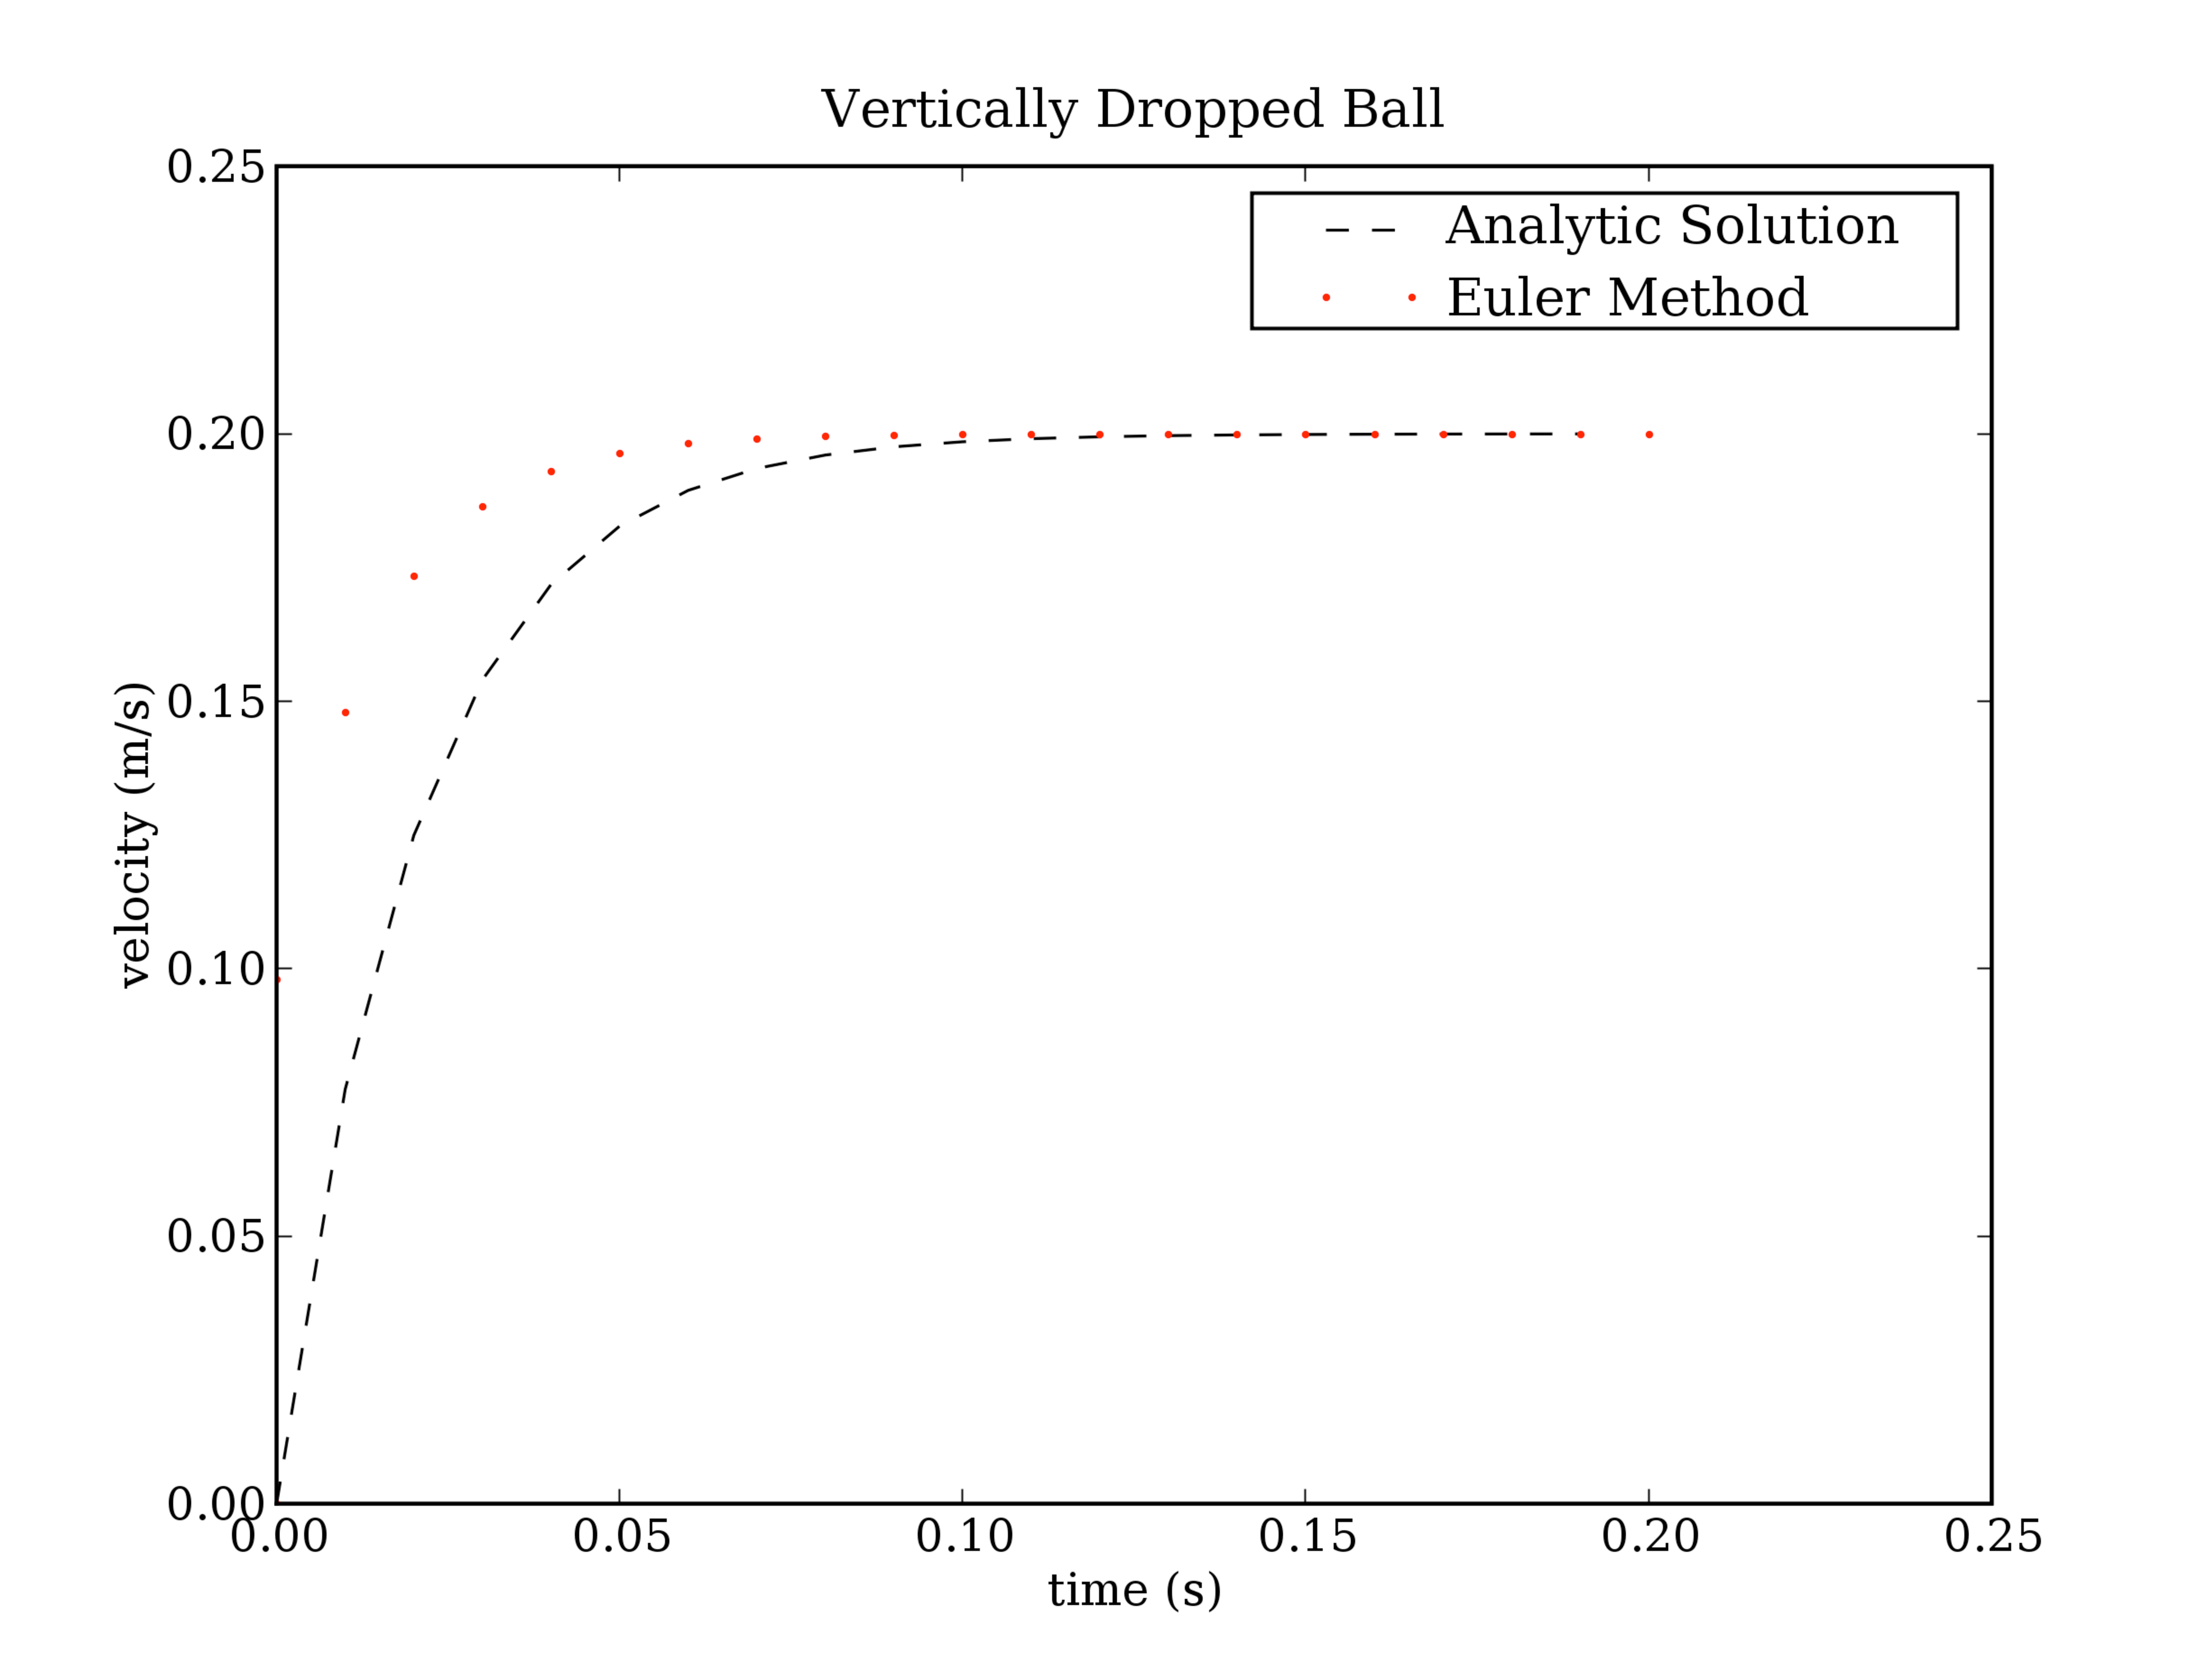
\includegraphics[height=8cm]{Figures/5Kinematics/glycerin}
\caption{Speed vs time for a 1.25 cm diameter ball bearing falling through glycerin at room temperature. Note that the time step is clearly too large,
since the simulation is clearly not a good fit to the analytic solution.}
\label{fig:glycerin}       % Give a unique label
\end{figure}

Notice that Figure~\ref{fig:glycerin} shows the exact (analytic) solution, as well as the simulated solution via the Euler Method. In running the simulation, the time step of 0.01 was clearly too large. This is evidenced by the poor disagreement with the analytic solution. In a situation such as this one, where the analytic solution is available, it is easy to make a comparison; however, we typically employ a computer simulation to solve a problem that is \textbf{not} analytically solvable. How do we decide on an appropriate time step then?

There are two answers to this question. First, we should always check our simulation's reasonableness by inputing parameters that are analytically solvable. For instance, in the previous problem, we can set the terminal velocity to be very large (ideally infinite, but a large number will do) and check to see that we recover the behavior of a ball falling freely in a gravitational field. Second, we can run the simulation with smaller and smaller time steps until the solutions converge upon one another. 

\subsection{Simulation of Linear Drag: \textsf{getopt} package}
\label{sec-LinDragGetOpt}

For example, here is Listing~\ref{code:FreeFallLinearDrag} modified in the following manner: 
\begin{itemize}
	\item We use the getopt (get options) package to parse (i.e. read in) the options passed from the command line.
	\item We add the ability to specify several different time steps (in fact, as many as you want!), and the code runs once for each one and plots all of them out, complete with a labeled legend.
\end{itemize}

\lstinputlisting[caption={This program uses the Euler method to solve for the velocity of a ball falling under the influence of a drag force proportional to the speed of fall. You may enter any number of different time steps, and the program will run once for each one. The program also uses the getopt package to parse input parameters.}, label=code:FreeFallGetOpt, frame=single]{Code/5Kinematics/FreeFallGetOpt.py}

The \textsf{getopt} package is designed to parse the input parameters from the command line; 
We use the previous input parameters to run the program: 
\begin{itemize}
	\item vinitial = 0.0
	\item vterminal = 0.2
	\item  tmax=0.2
	\item dt=0.01
\end{itemize}
and then add two more time steps (dt=0.001, and 0.0001), we run this program as follows:\\
\begin{verbatim}
python FreeFallGetOpt.py --filename junk --v_initial 0.0
--v_terminal 0.2 --tmax 0.2 0.01 0.001 0.0001
\end{verbatim}
and this produces the output shown in Figure~\ref{fig:freefallgetopt}
\begin{figure}[b]
\centering
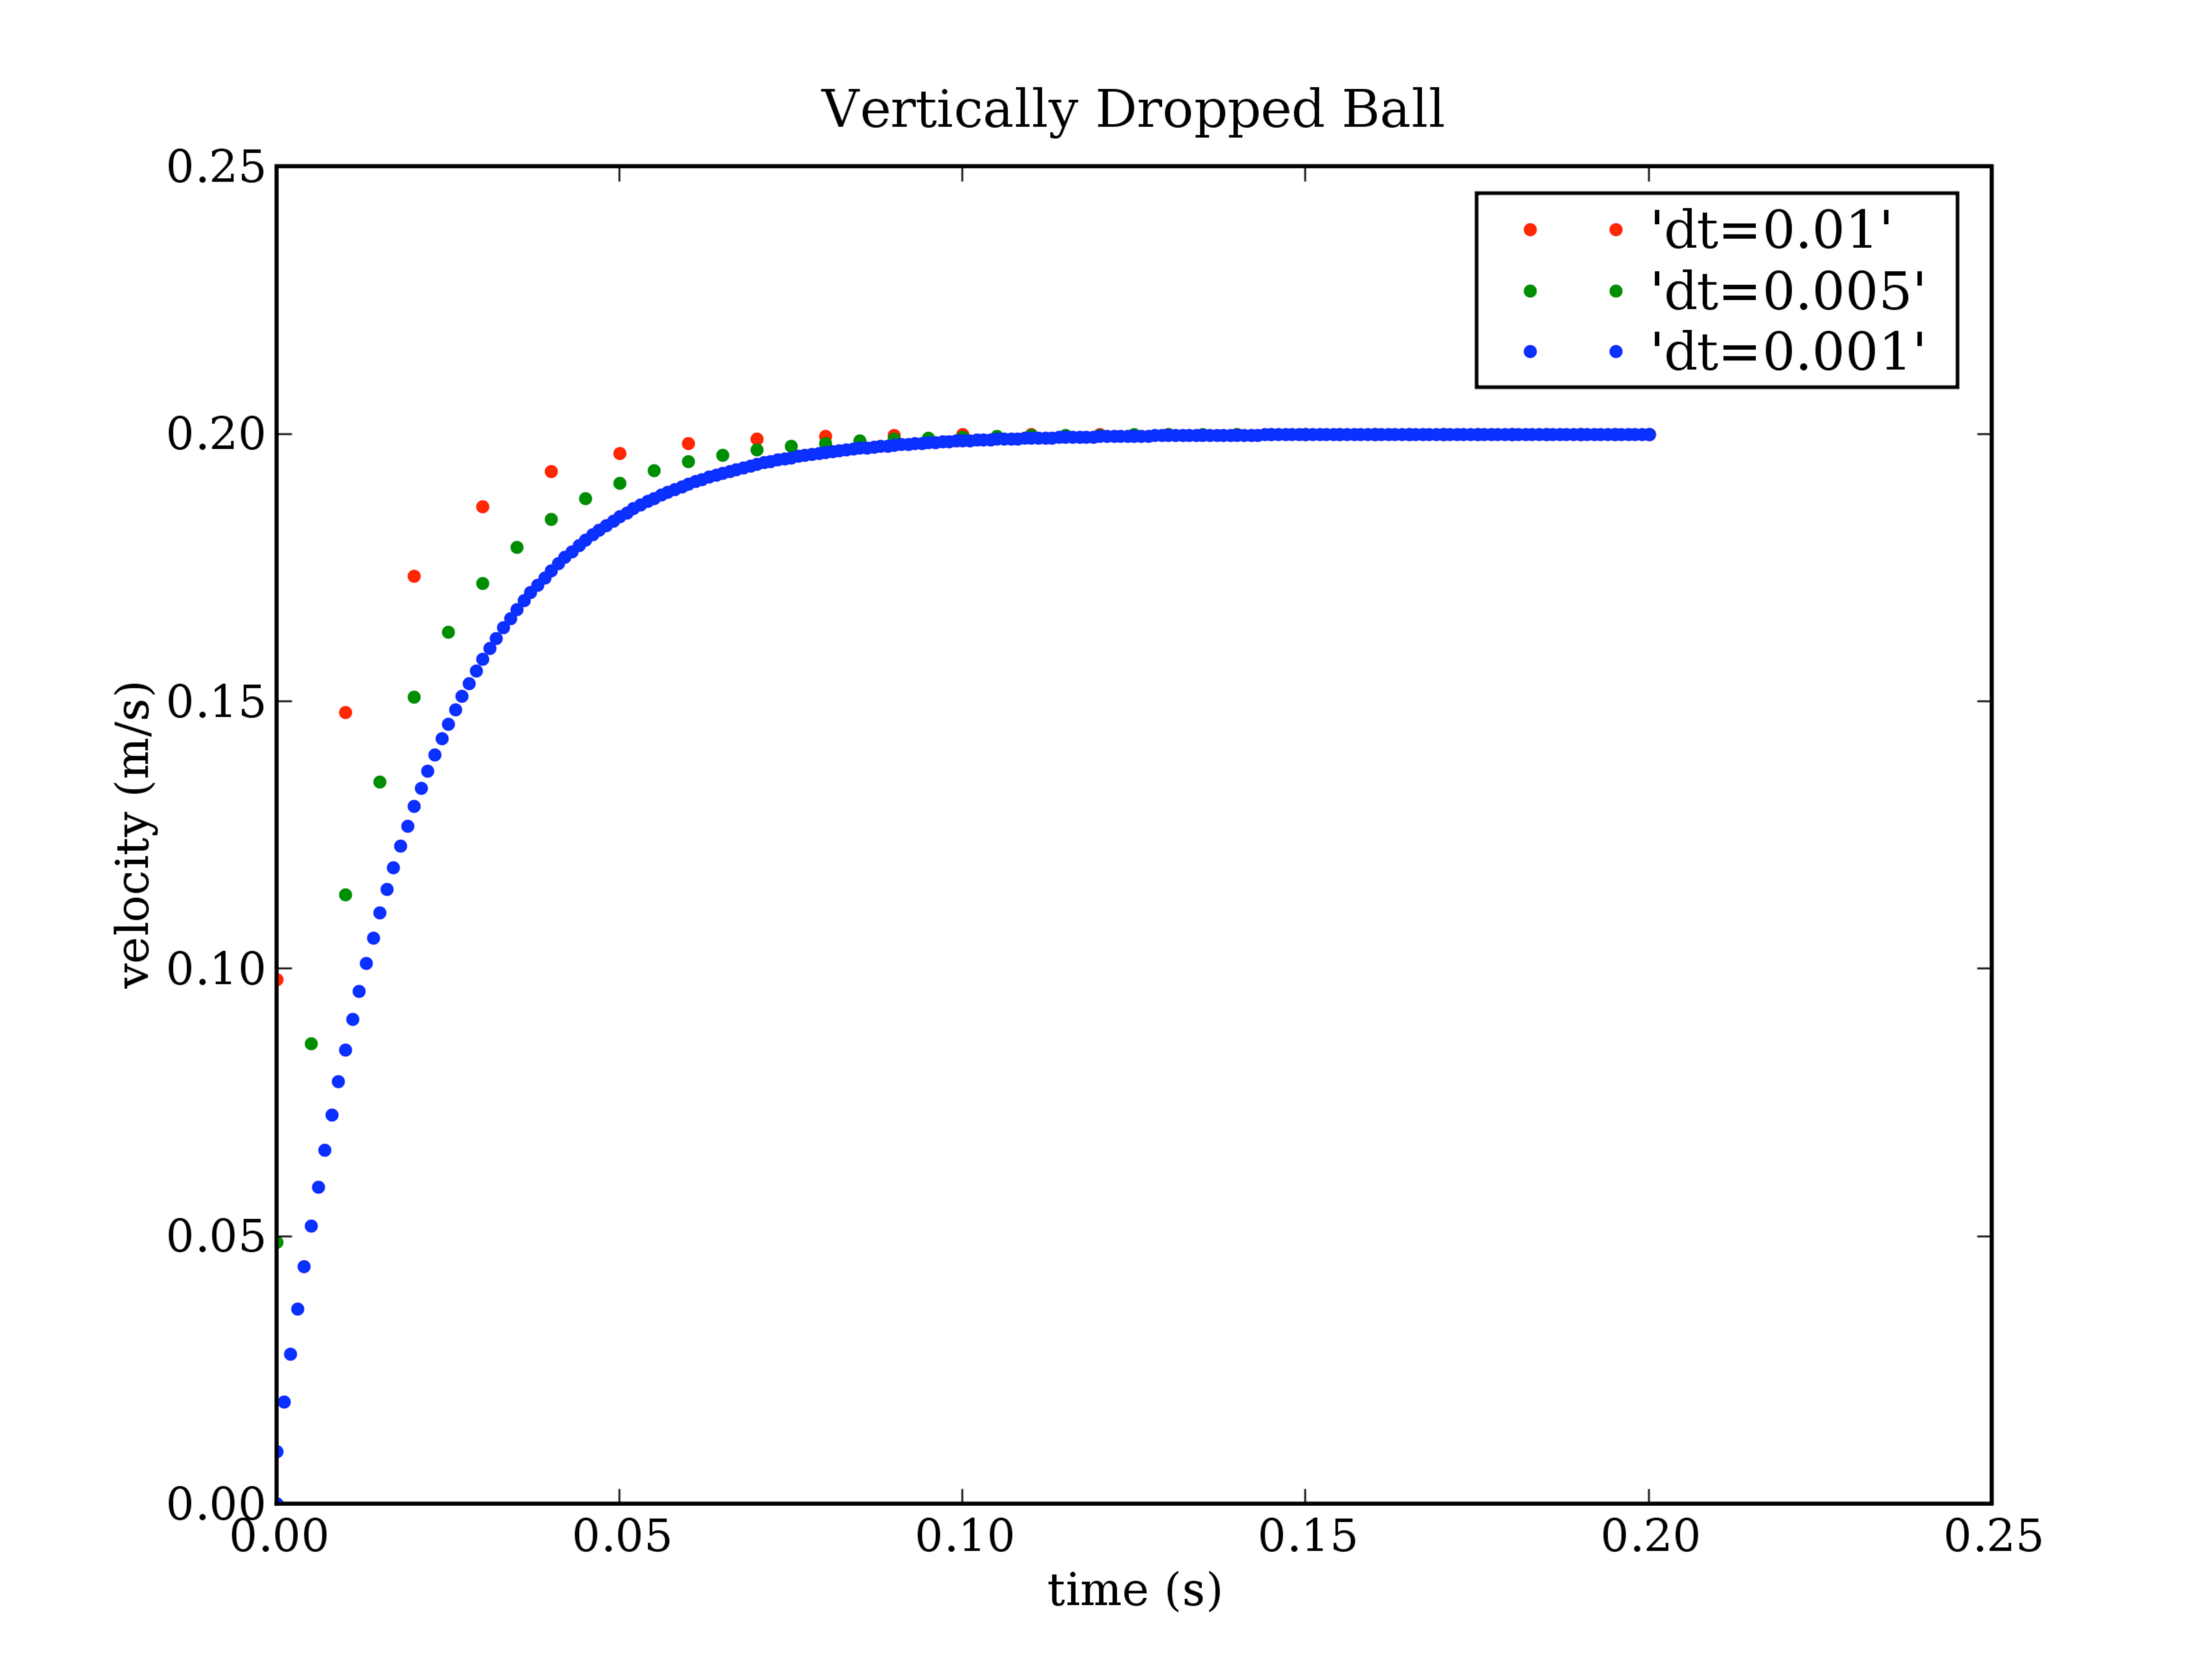
\includegraphics[height=7cm]{Figures/5Kinematics/getopt.pdf}
\caption{Speed vs time for a 1.25 cm diameter ball bearing falling through glycerin at room temperature; three different time steps are shown.}
\label{fig:freefallgetopt}       % Give a unique label
\end{figure}
The convergence of the simulation to the analytical result in this figure is very clear; in fact, a plot of the analytical result lies almost directly on top of the trial with dt=0.0001 seconds. 

\pagebreak
\subsection{Simulation of Linear Drag: \textsf{argparse} package}
\label{sec-LinDragArgParse}

\lstinputlisting[caption={This program uses the Euler method to solve for the velocity of a ball falling under the influence of a drag force proportional to the speed of fall. You may enter any number of different time steps, and the program will run once for each one. The program also uses the \textsf{argparse} package to parse input parameters.}, label=code:FreeFallArgParse, frame=single]{Code/5Kinematics/FreeFallArgParse.py}


\pagebreak
%
\section{Motion in Two Dimensions}
\label{sec-2d}
%
Now that we have solved a few one-dimensional problems, let's work out how to numerically integrate Newton's 2nd law for  motion in two dimensions. Building on our work modeling air resistance, let's reason out the physics for projectile motion with quadratic drag. 

At high velocities (technically, when the Reynolds number, R$_e  > 1000$), we can write the drag force, $F_\mathrm{D}$ on an object moving through a fluid of density $\rho$ as roughly
\begin{equation} 
\vec{F}_{\mathrm{D}} = - \frac{1}{2}\rho C_d A v^2\;\hat{v} 
\label{eq:drag}
\end{equation}
where 
$C_d$ is the drag coefficient (depends on velocity; 0.07 to 0.5 for a sphere, for example, $\approx 0.04$ for a plane, 0.25 to 0.45 for a car), $A$ is the cross-sectional area, and $v$ is the speed for the speed of the object through the fluid.

Notice, of course, that the drag force is always opposite the velocity, so we can draw the free-body diagram on (for example) a sphere as in Figure~\ref{fig:2DFreeBody}:
\begin{figure}
	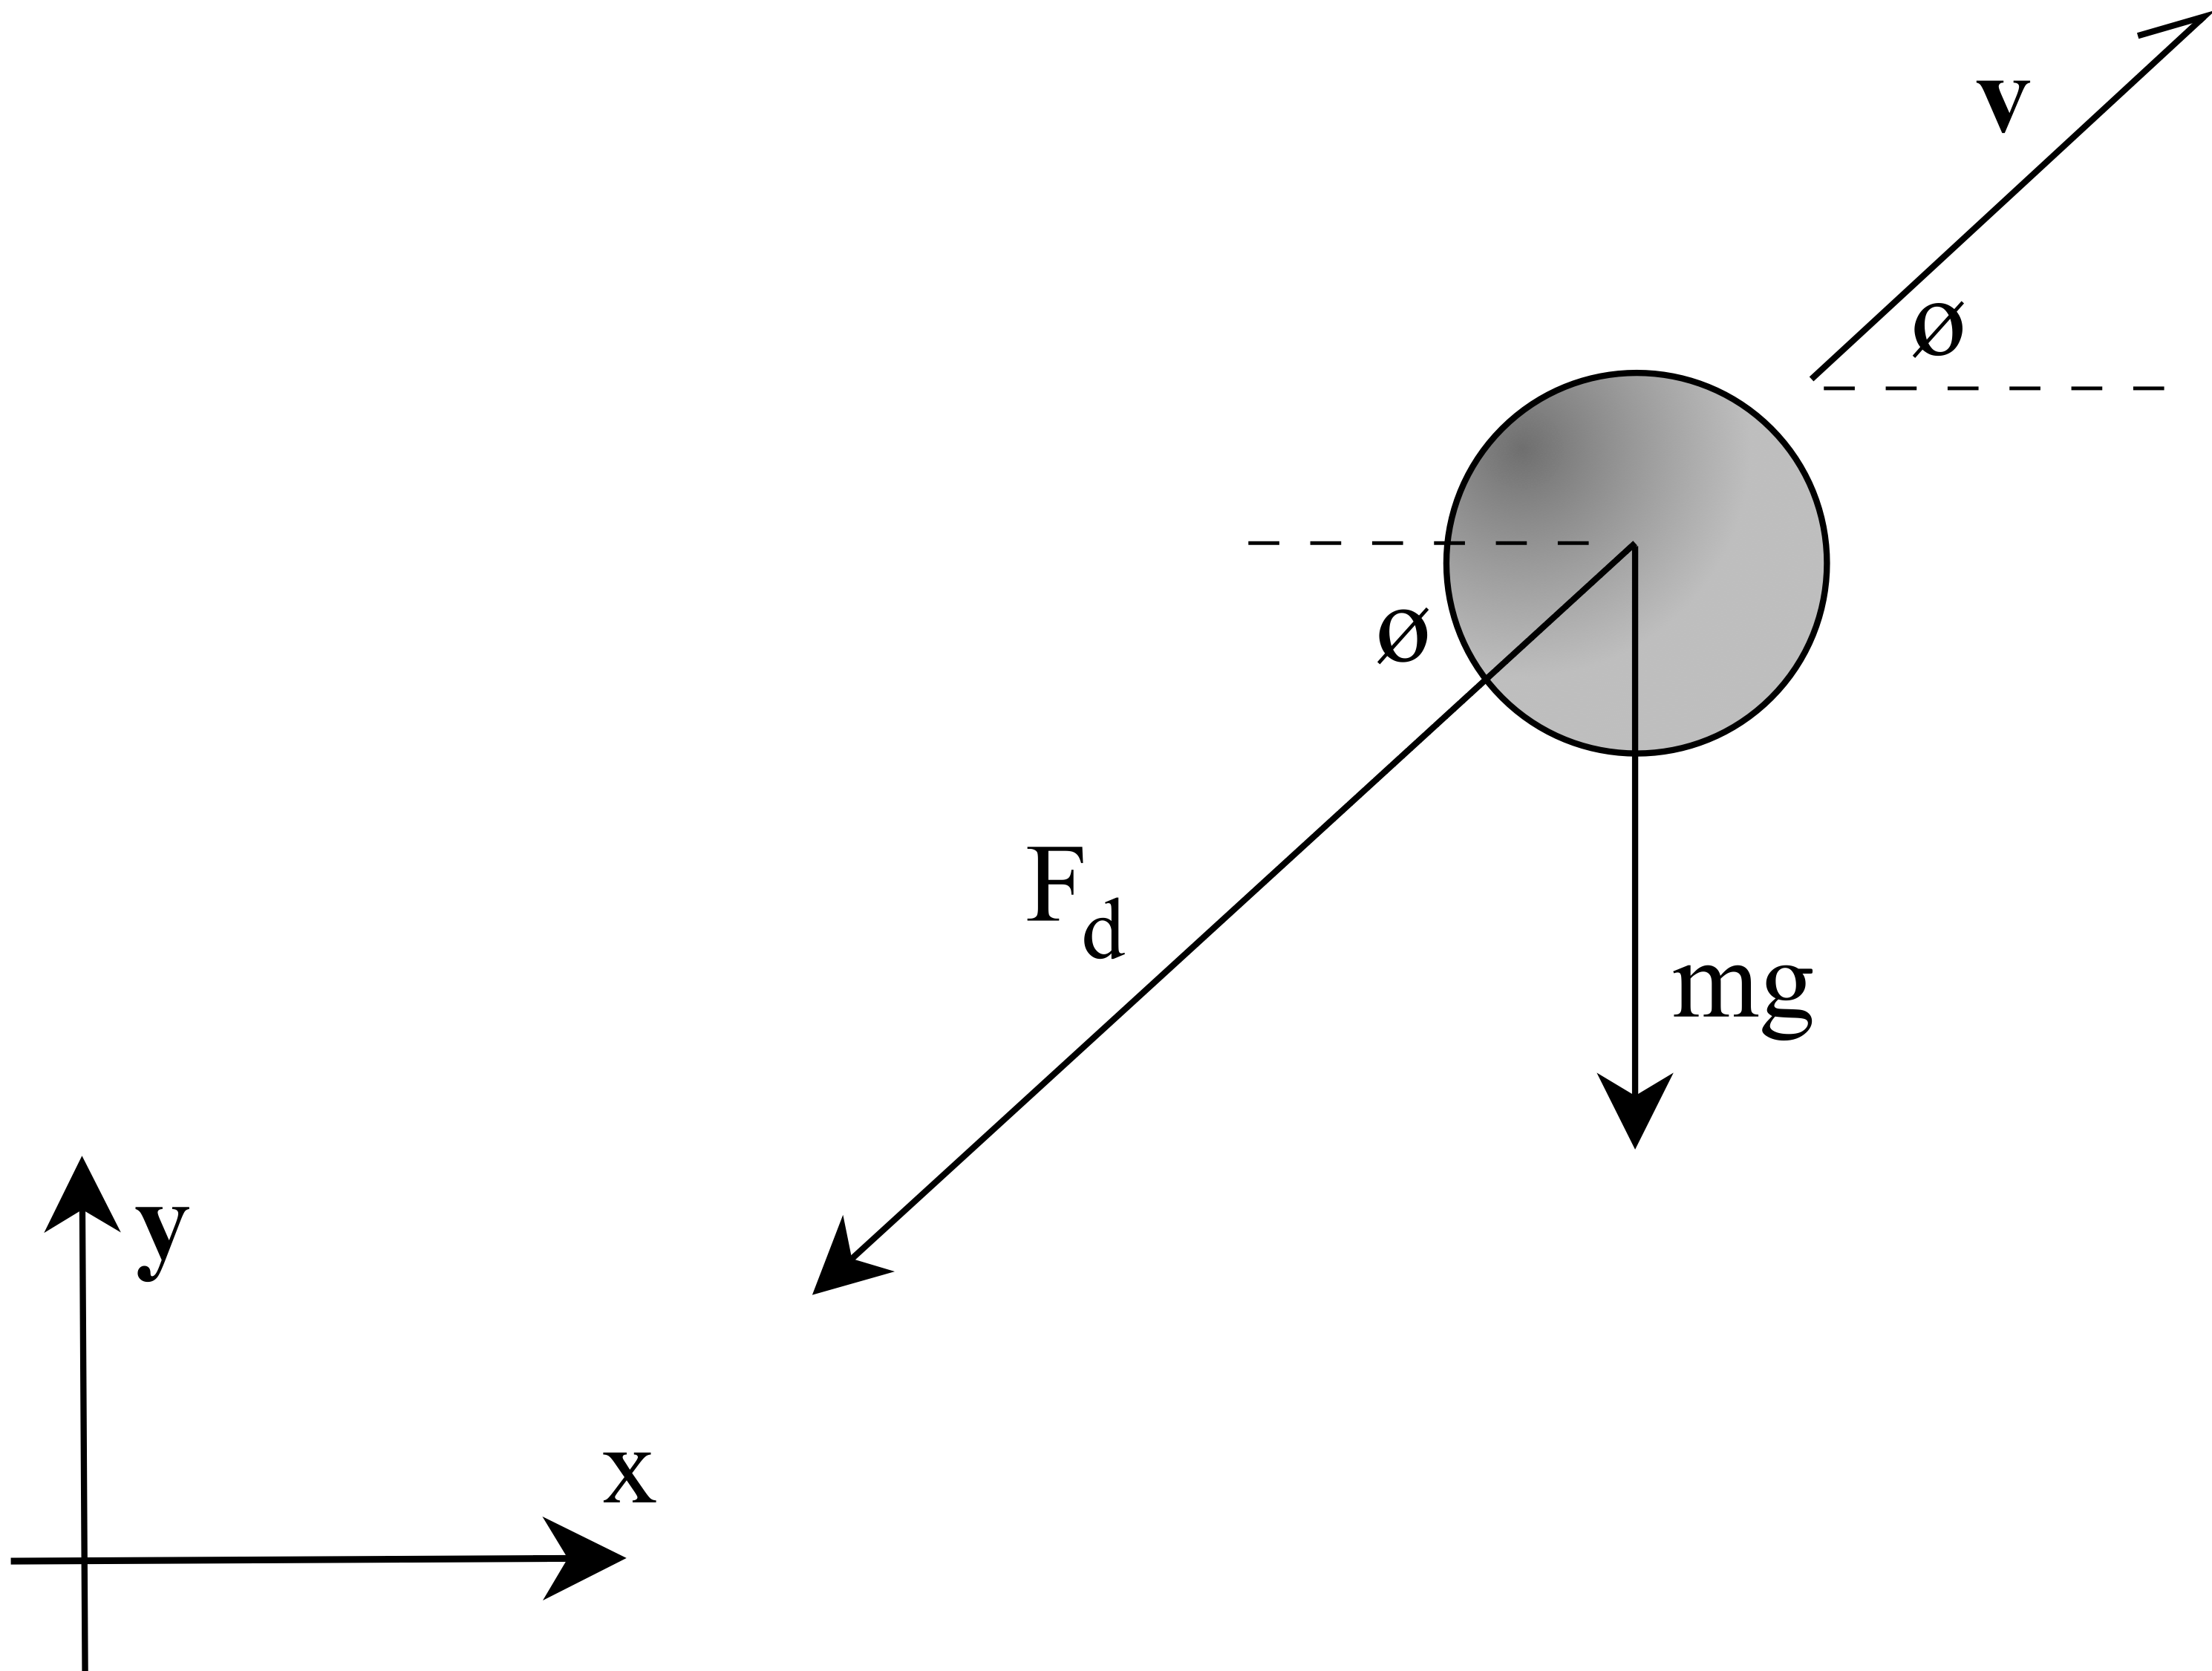
\includegraphics[width=3.5in]{Figures/5Kinematics/2DFreeBody.png}
	\caption{A sphere moving in two dimensions with air drag.}\label{fig:2DFreeBody}
\end{figure}

Now, let's consider a sphere traveling through the air with a drag force quadratic in the velocity and of the general form 
$$  \vec{F}_{\mathrm{D}} = - B v^2\;\hat{v}.   $$
Applying Newton's second law (using a Cartesian coordinate system) and keeping in mind that 
$$\hat{v} = \frac{\vec{v}}{v} = \frac{v_x \,\hat{\imath} + v_y \,\hat{\jmath}}{\sqrt{v_x^2 + v_y^2}}$$
we see that the drag force is 
$$  \vec{F}_{\mathrm{D}} = - B v\;\left(v_x \,\hat{\imath} + v_y \,\hat{\jmath}\right).    $$
and therefore Newton's second law in the x and y directions is 
$$ m \frac{dv_x}{dt} = -B v v_x $$
and 
$$  m \frac{dv_y}{dt} = -B v v_y -mg. $$

We can now write down the governing equations to simulate the motion using the Euler method: 
$$ x_{i+1} = x_i + v_{x_i} \Delta t $$
$$ y_{i+1} = y_i + v_{y_i} \Delta t $$
$$ v_{x_{i+1}} = v_{x_i} - \frac{B v_i v_{x_i}}{m}\Delta t $$
$$ v_{y_{i+1}} = v_{y_i} - \frac{B v_i v_{y_i}}{m}\Delta t - g\Delta t $$
where the speed, $v_i$ is 
$$v_i = \sqrt{v^2_{x_i} + v^2_{y_i}}$$
Notice that to update the x and y velocities, we need to know the value of $B/m$; so let's calculate this value assuming the simplest case of a sphere of density $\rho_s$ moving through air with density $\rho_a$. Notice that we can write equation~\ref{eq:drag} as
\begin{equation} 
\vec{F}_{\mathrm{D}} = - \frac{1}{2}\rho \,C_d A v^2 \;\hat{v} = -B \, v^2 \;\hat{v}
\label{eq:dragModified}
\end{equation}
where $B=\frac{1}{2}\rho \,C_d A$ and therefore a sphere with cross-sectional area $A = \pi R^2$, has 
\begin{equation}
	\frac{B}{m} = \frac{\frac{1}{2}\rho_a C_d \pi R^2}{\frac{4}{3}\pi R^3 \rho_s}
\end{equation}
If we make the assumption that $C_d = \frac{1}{2}$ for the drag coefficient, then we have 
\begin{equation} 
	\frac{B}{m} = \frac{3}{16} \frac{\rho_a}{\rho_s} \, \frac{1}{R}
\end{equation}


\pagebreak 

% Problems or Exercises should be sorted chapterwise
\section*{Problems}
\addcontentsline{toc}{section}{Problems}
%
% Use the following environment.
% Don't forget to label each problem;
% the label is needed for the solutions' environment

\begin{prob}
\label{prob2.1}
Modify the program \textsf{Falling Ball} to correctly deal with air resistance that is proportional to the square of the velocity. This is the air resistance that is a better model for objects such as bowling balls falling from the tops of buildings.  
The magnitude of the air drag, $F_d$ in this case is 
$$ F_d = b_2 v^2 $$
where $b_2$ is a constant that (in general) must be determined empirically. If a ball is dropped and allowed to achieve terminal velocity, then the drag force will be equal to the pull of gravity, and we will have
$$ mg = b_2 v_{t}^2$$
and therefore, the constant $b_2$ will be 
$$ b_2 = \frac{mg}{v_{t}^2},$$
which allows us to rewrite the drag force in terms of the terminal velocity:
$$ F_d = mg \left(\frac{v}{v_t}\right)^2 $$
Let's assume that we have a ball of radius 0.01 m, where the terminal velocity in air is found to be about 30 m/s. Now, following the reasoning in Section~\ref{sec-LinDragSimulation}, modify the code in program \textsf{Falling Ball} to use quadratic air resistance (also referred to as inertial drag), and compute the speed at which this ball reaches the ground if it is dropped from rest from a height of 100 m. Compare this speed to a a freely falling object with no air resistance. 
\end{prob}

\begin{prob}
\label{2d}
Simulate the motion of three objects:
\begin{enumerate}
	\item A steel ball with density 8000 kg/m$^3$ traveling through vacuum.
	\item A 2 cm diameter steel ball with density 8000 kg/m$^3$ traveling through air of density 1.2 kg/m$^3$
	\item A  2 cm balsa wood ball with density 160 kg/m$^3$ traveling through air of density 1.2 kg/m$^3$
\end{enumerate}
a) Make sure to test that your simulation for the zero air resistance case agrees with basic kinematics (it goes without saying that you should do this!) and check to see that the other two situations give sensible results. \\
Using an initial velocity of 100 m/s and a launch angle of $30^o$: \\
b) Make a plot of y .vs. x for the three scenarios.\\
c) Plot the total mechanical energy .vs. time for the three scenarios. Discuss this plot in your report. Does the Euler method properly conserve energy for the zero air resistance case? \\
Lastly, \\
(d) modify your program to find the launch angle that gives the maximum range for the steel ball and the balsa wood ball. Assume that the initial launch speed is 100 m/s. 
Write all this up using the LaTeX report template. Follow the guidelines closely; the quality of the writing in the report is important. I'll reject it and return it to you if it's poorly written, and you'll have to re-submit your report.\\


\end{prob}


%
